\documentclass[11pt]{article}

% -----------------------------
% Preambula
% -----------------------------
\usepackage[slovene]{babel}       
\usepackage[utf8]{inputenc}       
\usepackage[T1]{fontenc}          
\usepackage{amsmath, amsthm}      
\usepackage{amssymb}              
\usepackage{graphicx}             

% AMS okruženja
\newtheorem{definicija}{Definicija}[section]
\newtheorem{izrek}{Izrek}[section]

% Komanda \f
\newcommand{\f}{\mathcal{F}}

% Naslov i autor
\title{Brownovo gibanje}
\author{Matej Rojec}
\date{}

% -----------------------------
\begin{document}
\maketitle

% =============================
% UVOD
% =============================
\section{Uvod}
Brownovo gibanje (več v \cite{karatzas1991brownian}) je intuitivno slučajen proces, ki predstavlja naključno gibanje delcev v mediju.

% =============================
% SLIKA
% =============================
\begin{figure}[h]
\centering
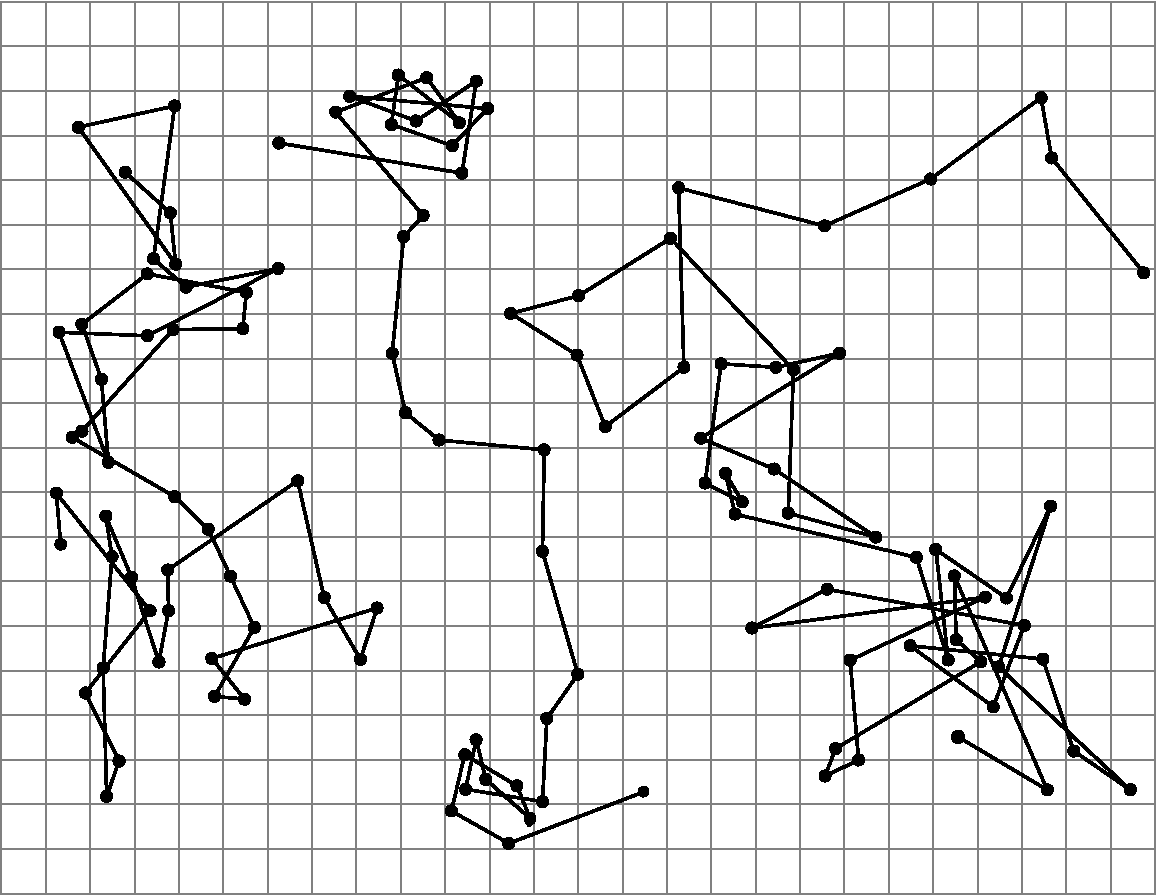
\includegraphics[width=0.5\textwidth]{PerrinPlot2.pdf}
\caption{Reprodukcija slike iz Jean Baptiste Perrin, \emph{Mouvement brownien et réalité moléculaire}, Ann. de Chimie et de Physique (VIII) 18, 5-114, 1909}
\label{fig:perrinplot}
\end{figure}

% =============================
% DEFINICIJE
% =============================
\section{Definicije}

\begin{definicija}[Standardno Brownovo gibanje]
Standardno Brownovo gibanje $\{B_t\}_{t \geq 0}$ je slučajen proces z naslednjimi lastnostmi: 
\begin{itemize}
\item $B_0 = 0$,
\item Prirastki $B_{t_n} - B_{t_{n-1}}, B_{t_{n-1}} - B_{t_{n-2}}, \ldots, B_2 - B_1, B_1 - B_0$ so neodvisne slučajne spremenljivke za vsak $t_0 \le t_1 \le \cdots \le t_n$,
\item Za vsak $t \ge 0$ in $h > 0$ velja $B_{t+h} - B_t \sim \mathcal{N}(0, h)$,
\item Funkcija $t \mapsto B_t$ je zvezna skoraj gotovo.
\end{itemize}
\end{definicija}

\begin{definicija}[Čas ustavljanja]
Slučajna spremenljivka $\tau$ na verjetnostnem prostoru $(\Omega, \mathcal{F}, P)$ z vrednostmi v $\mathbb{R}^+$ je čas ustavljanja glede na filtracijo $(\f_t)_{t \in T}$, če velja: 
\[
\forall t \in T: \{\tau \le t\} \in \f_t.
\]
\end{definicija}

% =============================
% IZREK
% =============================
\section{Izrek}

\begin{izrek}[Sklep o ustavljenem Brownovem gibanju]\label{thm:stopped_brownian}
Naj bo $\{B_t\}_{t \geq 0}$ standardno Brownovo gibanje, $\tau$ čas ustavljanja glede na $(\f_t)_{t \ge 0}$ in naj velja $P[\tau < \infty] = 1$.  
Potem je tudi proces
\[
\hat{B} := \{B_{T+t} - B_T \mid t \geq 0\}
\]
standardno Brownovo gibanje in neodvisen od $\f_T$.
\end{izrek}

V besedilu se na izrek sklicujemo kot \ref{thm:stopped_brownian}.

% =============================
% Literatura
% =============================
\bibliographystyle{plain}
\bibliography{knjiga}

\end{document}
